\begin{figure}[t]
\centering
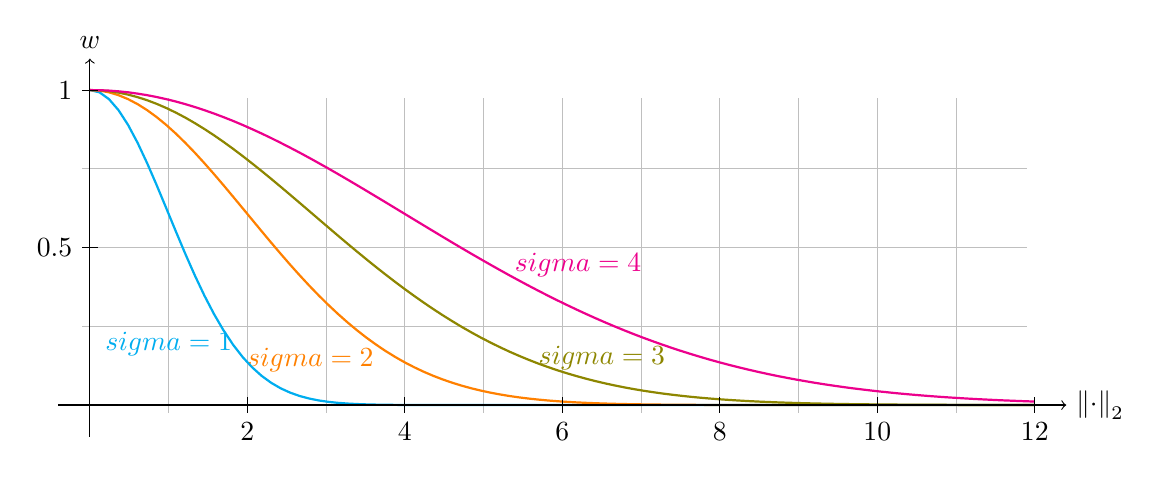
\begin{tikzpicture}
  \draw[color=lightgray] (-0.1, -0.1) grid (11.9, 3.9);
  \tikzstyle{color1}=[color=cyan]
  \tikzstyle{color2}=[color=orange]
  \tikzstyle{color3}=[color=olive]
  \tikzstyle{color4}=[color=magenta]

  \draw[color1] (1,0.5) node[above]   {$\gls{sigma} = 1$};
  \draw[color2] (2.8,0.3) node[above] {$\gls{sigma} = 2$};
  \draw[color3] (6.5,0.32) node[above] {$\gls{sigma} = 3$};
  \draw[color4] (6.2,1.5) node[above] {$\gls{sigma} = 4$};

  \draw [color1, thick,domain=0:12, samples=100] plot (\x,4*exp{-(\x)^2/2});  % 1
  \draw [color2, thick,domain=0:12, samples=100] plot (\x,4*exp{-(\x)^2/8});  % 2
  \draw [color3, thick,domain=0:12, samples=100] plot (\x,4*exp{-(\x)^2/16});  % 3
  \draw [color4, thick,domain=0:12, samples=100] plot (\x,4*exp{-(\x)^2/32});  % 4

  \draw[->] (-0.4, 0) -- (12.4, 0) node[right] {${\left\|\cdot\right\|}_2$};
  \draw[->] (0, -0.4) -- (0, 4.4) node[above] {$w$};
  \draw (0.1, 2) -- (-0.1, 2) node[left] {$0.5$};
  \draw (0.1, 4) -- (-0.1, 4) node[left] {$1$};
  \draw (2, 0.1) -- (2, -0.1) node[below] {$2$};
  \draw (4, 0.1) -- (4, -0.1) node[below] {$4$};
  \draw (6, 0.1) -- (6, -0.1) node[below] {$6$};
  \draw (8, 0.1) -- (8, -0.1) node[below] {$8$};
  \draw (10, 0.1) -- (10, -0.1) node[below] {$10$};
  \draw (12, 0.1) -- (12, -0.1) node[below] {$12$};

\end{tikzpicture}
  \caption[Kantengewichtsberechnung über Gaußfunktion]{Illustration der \enquote{invertierten} Kantengewichte $w \in \left[0, 1\right]$ basierend auf dessen Länge, gegeben durch die euklidische Norm ${\left\|\cdot\right\|}_2$.
  Je größer $\gls{sigma} \in \gls{R}$ gewählt, umso \enquote{stumpfer} zeichnet sich die Gaußfunktion und umso längere Kanten erhalten ein Gewicht $\gg 0$.}
\label{fig:gauss}
\end{figure}
